% !TeX spellcheck = en_US
% !TeX encoding = UTF-8
\section{Enveloping distribution sampling\label{Sec:ES:EDS}}
Enveloping distribution sampling method was first proposed by Christ and van Gunsteren in 2007.\cite{ChristJCP2007}.
When calculating the free energy difference between states $A$ and $B$,
\begin{equation}
	\Delta G_{BA}=G_B-G_A=-\beta^{-1}\ln{\frac{Q_B}{Q_A}},
\end{equation}
we may encounter convergence difficulty if the important spaces of these two states are well separated, shown as black lines in Fig.~\ref{Fig:ES:triple_gaussian}.
Simulation under the Hamiltonian of state $A$ can hardly cover the important region of Hamiltonian $B$, and then the free energy of state $B$ will be significantly overestimated.
\begin{figure}[htbp]
	\centering
	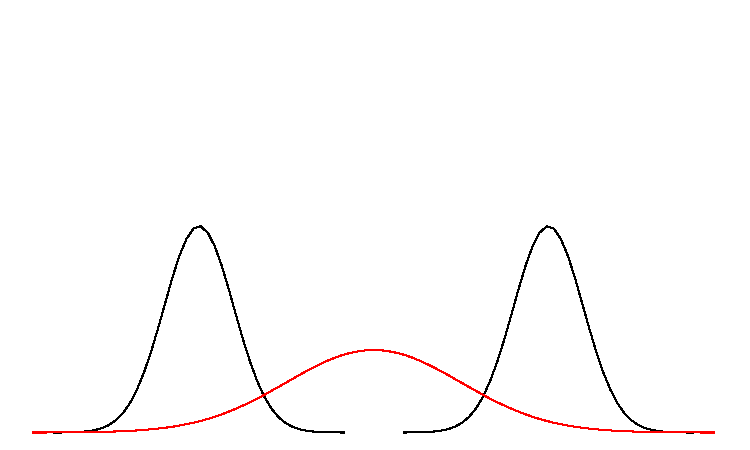
\includegraphics[width=0.6\textwidth]{figures/triple_gaussian.pdf}\\
	\caption{}\label{Fig:ES:triple_gaussian}
\end{figure}
A simple solution to this difficulty is ``overlap sampling'', in which a reference state that can cover the important regions of both Hamiltonians $A$ and $B$ is introduced.
We then carry out a simulation for the reference state and the free energy difference between state $A$ and $B$ can be calculated as
\begin{equation}
	\Delta G_{BA}=\Delta G_{BR}-\Delta G_{AR}=-\beta^{-1}\ln{\frac{\left<e^{-\beta\left(H_B-H_R\right)}\right>_R}{\left<e^{-\beta\left(H_A-H_R\right)}\right>_R}},
\end{equation} 
which is a combination of two thermodynamic perturbation calculations from the reference state to the target states.

However, building the Hamiltonian of the reference state is not trivial. Without knowledge of the Hamiltonians for state $A$ and state $B$, we cannot generate an effective Hamiltonian,
especially in a high dimensional space. Enveloping distribution sampling method provides a natural way to generate the Hamiltonian for the reference state with simply mixing the Hamiltonians of state $A$ and state $B$ in the following way
\begin{equation}
	H_R(\mathbf{r})=-\left(s\beta\right)^{-1}\ln{\left(e^{-s\beta H_A(\mathbf{r})}+e^{-s\beta H_B(\mathbf{r})}\right)},
\end{equation}
where $s$ is a scale factor that modulates the mixing\cite{ChristJCTC2009} as shown in Fig.~\ref{Fig:ES:EDS}. Increasing $s$ lows the barrier height separating the two minima in the mixed potential, thereby enhances the transition. Quite straightforward, you may come to the idea that running Hamiltonian-REMD with different $s$ can remarkably increase the efficiency.

\begin{figure}[htbp]
	\centering
	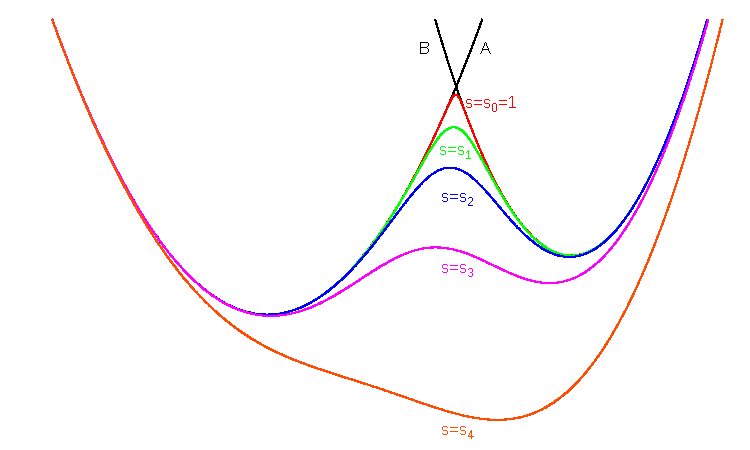
\includegraphics[width=0.8\textwidth]{figures/EDS.pdf}\\
	\caption{}\label{Fig:ES:EDS}
\end{figure}

The force is also a mixing from two Hamiltonians as
\begin{align}
	\mathbf{F}_R^i=-\frac{\partial H_R}{\partial \mathbf{r}^i}=&\frac{e^{-s\beta H_A(\mathbf{r})}}{e^{-s\beta H_A(\mathbf{r})}+e^{-s\beta H_B(\mathbf{r})}}\left(-\frac{\partial H_A(\mathbf{r})}{\partial \mathbf{r}^i}\right)\notag\\
	&+\frac{e^{-s\beta H_A(\mathbf{r})}}{e^{-s\beta H_B(\mathbf{r})}+e^{-s\beta H_B(\mathbf{r})}}\left(-\frac{\partial H_B(\mathbf{r})}{\partial \mathbf{r}^i}\right).
\end{align}
